\begin{center}
  \section*{Homework 13 - 8.2, 8.3}
  Due Wed 5/07 \\
  Uzair Hamed Mohammed
\end{center}

\subsection*{8.2 Discrete Least Squares Approximation}

3 (degree 2 only), 4 (degree 2 only), 9.

\begin{enumerate}
  \item[3.] Find the least square polynomials of degree 2 for the
    data in the following table. Compute the error \(E_2\) in each
    case. Graph the data and the polynomials.

    \[
      \begin{array}{lcccccc}
        \hline
        x_i & 1.0 & 1.1 & 1.3 & 1.5 & 1.9 & 2.1 \\
        y_i & 1.84 & 1.96 & 2.21 & 2.45 & 2.94 & 3.18 \\
        \hline
      \end{array}
    \]

    \underline{Sol}:\\

    Normal equations:
    \[
      \begin{bmatrix}
        6 & 8.9 & 14.17 \\
        8.9 & 14.17 & 24.023 \\
        14.17 & 24.023 & 42.8629
      \end{bmatrix}
      \begin{bmatrix}
        a_0 \\ a_1 \\ a_2
      \end{bmatrix}
      =
      \begin{bmatrix}
        14.58 \\ 22.812 \\ 38.0862
      \end{bmatrix}
    \]

    Gaussian elimination steps:

    1. Eliminate \(a_0\):
    \[
      \begin{bmatrix}
        8.9 & 14.17 & 24.023 \\
        14.17 & 24.023 & 42.8629
      \end{bmatrix}
      -
      \begin{bmatrix}
        8.9 & 13.2017 & 20.9688 \\
        14.17 & 21.0188 & 33.4748
      \end{bmatrix}
      =
      \begin{bmatrix}
        0 & 0.9683 & 3.0542 \\
        0 & 3.0042 & 9.3881
      \end{bmatrix}
    \]
    \[
      \begin{cases}
        0.9683a_1 + 3.0542a_2 = 1.185 \\
        3.0042a_1 + 9.3881a_2 = 3.6631
      \end{cases}
    \]

    2. Eliminate \(a_1\):
    \[
      3.0042a_1 + 9.3881a_2 - 3.102 \times (0.9683a_1 + 3.0542a_2) =
      3.6631 - 3.102 \times 1.185
    \]
    \[
      -0.0839a_2 = -0.0129 \quad \Rightarrow \quad a_2 =
      \frac{-0.0129}{-0.0839} \approx 0.1537
    \]

    3. Back-substitute \(a_2\):
    \[
      0.9683a_1 + 3.0542(0.1537) = 1.185 \quad \Rightarrow \quad a_1
      \approx 1.7558
    \]

    4. Back-substitute \(a_1, a_2\):
    \[
      6a_0 + 8.9(1.7558) + 14.17(0.1537) = 14.58 \quad \Rightarrow
      \quad a_0 \approx 0.2389
    \]

    Error \(E_2\):
    \[
      E_2 = \sum_{i=1}^6 \left(y_i - (0.2389 + 1.7558x_i -
      0.1752x_i^2)\right)^2 \approx 0.0022
    \]

    \[
      \boxed{P(x) = 0.239 + 1.756x - 0.175x^2} \quad \boxed{E_2 \approx 0.0022}
    \]

    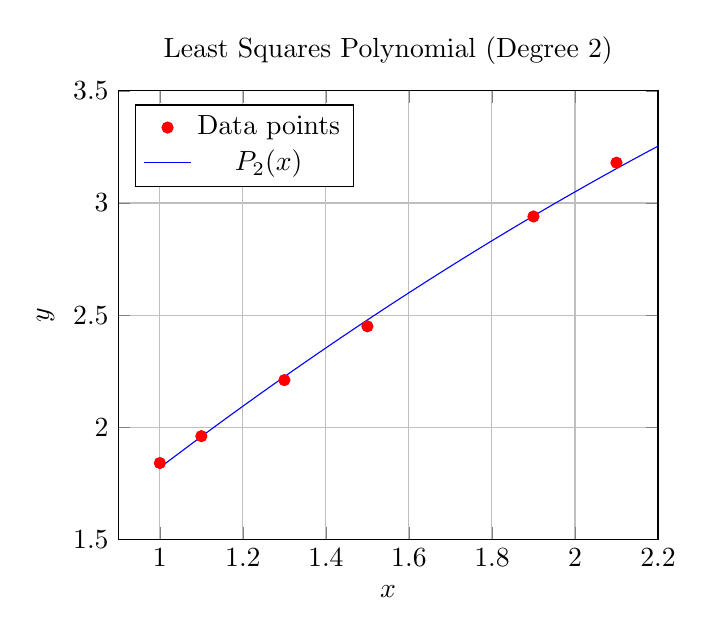
\begin{tikzpicture}
      \begin{axis}[
          title={Least Squares Polynomial (Degree 2)},
          xlabel={$x$},
          ylabel={$y$},
          xmin=0.9, xmax=2.2,
          ymin=1.5, ymax=3.5,
          grid=both,
          legend pos=north west
        ]

        % Data points
        \addplot[only marks, mark=*, red] coordinates {
          (1.0, 1.84)
          (1.1, 1.96)
          (1.3, 2.21)
          (1.5, 2.45)
          (1.9, 2.94)
          (2.1, 3.18)
        };

        % Polynomial P(x) = 0.2389 + 1.7558x - 0.1752x²
        \addplot[blue, domain=1:2.2, smooth] {
          0.2389 + 1.7558*x - 0.1752*x^2
        };
        \legend{Data points, $P_2(x)$}
      \end{axis}
    \end{tikzpicture}

  \item[4.] Find the least square polynomials of degree 2 for the
    data in the following table. Compute the error \(E_2\) in each
    case. Graph the data and the polynomials.

    \[
      \begin{array}{lcccccc}
        \hline
        x_i & 0 & 0.15 & 0.31 & 0.5 & 0.6 & 0.75 \\
        y_i & 1.0 & 1.004 & 1.031 & 1.117 & 1.223 & 1.42 \\
        \hline
      \end{array}{l}
    \]

    \underline{Sol}:\\

    \[
      \begin{bmatrix}
        6 & 2.31 & 1.2911 \\
        2.31 & 1.2911 & 0.796041 \\
        1.2911 & 0.796041 & 0.5182475
      \end{bmatrix}
      \begin{bmatrix}
        a_0 \\ a_1 \\ a_2
      \end{bmatrix}
      =
      \begin{bmatrix}
        6.795 \\ 2.82751 \\ 1.63997
      \end{bmatrix}
    \]

    \[
      \begin{bmatrix}
        a_0 \\ a_1 \\ a_2
      \end{bmatrix}
      =
      \begin{bmatrix}
        1.010 \\
        -0.320 \\
        1.137
      \end{bmatrix}
    \]

    \[
      P(x) = 1.010 - 0.320x + 1.137x^2
    \]

    \[
      E_2 = \sum_{i=1}^6 (y_i - P(x_i))^2 = 0.00091
    \]

    \[
      \boxed{P(x) = 1.010 - 0.320x + 1.137x^2} \quad \boxed{E_2 \approx 0.00091}
    \]

    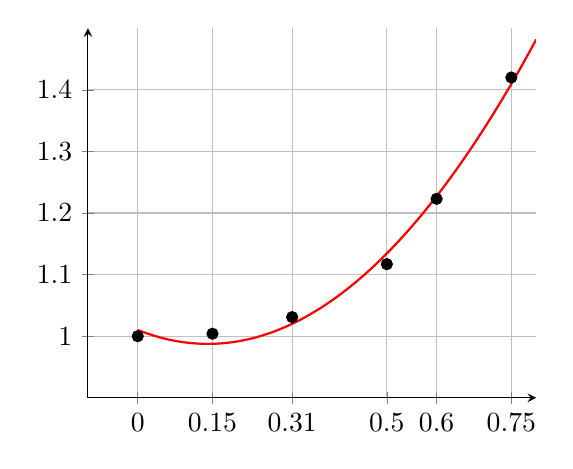
\begin{tikzpicture}
      \begin{axis}[
          xmin=-0.1, xmax=0.8, ymin=0.9, ymax=1.5,
          grid=both, axis lines=left,
          xtick={0,0.15,0.31,0.5,0.6,0.75},
          ytick={1.0,1.1,...,1.4},
          width=0.6\textwidth
        ]
        \addplot[only marks, mark=*, black] coordinates {
          (0,1.0) (0.15,1.004) (0.31,1.031)
          (0.5,1.117) (0.6,1.223) (0.75,1.42)
        };
        \addplot[red, domain=0:0.8, smooth, thick] {1.010 - 0.320*x +
        1.137*x^2};
      \end{axis}
    \end{tikzpicture}

  \item[9.] The following table lists the college grade-point
    averages of 20 mathematics and computer science majors, together
    with the scores that these students received on the mathematics
    portion of the ACT (American College Testing Program) test while
    in high school. Plot these data, and find the equation of the
    least squares line for this data. Do you think that the ACT
    scores are a reasonable predictor of college grade-point averages?

    \[
      \begin{array}{cccc}
        \hline
        \textrm{ACT Score} & \textrm{Grade-Point Average} &
        \textrm{ACT Score} & \textrm{Grade-Point Average} \\
        \hline
        28 & 3.84 & 29 & 3.75 \\
        25 & 3.21 & 28 & 3.65 \\
        28 & 3.23 & 27 & 3.87 \\
        27 & 3.63 & 29 & 3.75 \\
        28 & 3.75 & 21 & 1.66 \\
        33 & 3.20 & 28 & 3.12 \\
        28 & 3.41 & 28 & 2.96 \\
        29 & 3.38 & 26 & 2.92 \\
        23 & 3.53 & 30 & 3.10 \\
        27 & 2.03 & 24 & 2.81 \\
        \hline
      \end{array}
    \]

    \underline{Sol}:\\

    \[
      \begin{array}{l}
        n = 20,\quad \sum x = 546,\quad \sum y = 64.80, \\
        \sum xy = 1781.97,\quad \sum x^2 = 15034, \\
        b = \dfrac{20(1781.97) - 546(64.80)}{20(15034) - 546^2} = 0.101, \\
        a = \dfrac{64.80 - 0.101 \times 546}{20} = 0.487, \\
        \boxed{y = 0.487 + 0.101x} \\
        \boxed{\textrm{No, ACT scores are not a reasonable predictor
        of college grade-point averages}}
      \end{array}
    \]

    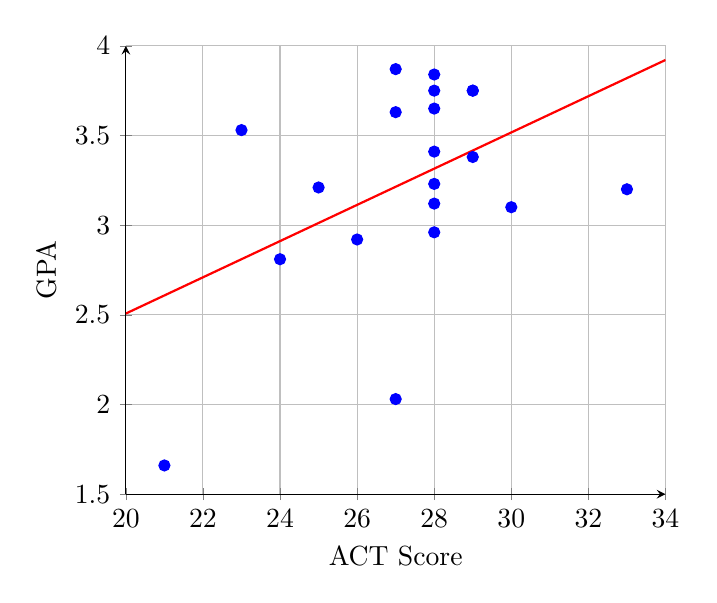
\begin{tikzpicture}
      \begin{axis}[
          xlabel=ACT Score, ylabel=GPA,
          xmin=20, xmax=34, ymin=1.5, ymax=4,
          grid=both, axis lines=left
        ]
        \addplot[only marks, mark=*, blue] coordinates {
          (28,3.84)(25,3.21)(28,3.23)(27,3.63)(28,3.75)(33,3.20)
          (28,3.41)(29,3.38)(23,3.53)(27,2.03)(29,3.75)(28,3.65)
          (27,3.87)(29,3.75)(21,1.66)(28,3.12)(28,2.96)(26,2.92)
          (30,3.10)(24,2.81)
        };
        \addplot[red, domain=20:34, thick]{0.487 + 0.101*x};
      \end{axis}
    \end{tikzpicture}

\end{enumerate}

\subsection*{8.3 Continuous Least Squares Approximation}

2e, 10, 11b

\begin{enumerate}
  \item[2.] Find the least square polynomial approximation of degree
    2 to the following function and interval.
    \begin{enumerate}
      \item[e.] \(f(x) = \frac{1}{2} \cos x + \frac{1}{3} \sin 2x\)

        \underline{Sol}:\\

        \[
          \begin{array}{l}
            \text{Interval: } [-\pi, \pi] \\
            \text{Inner product: } \langle f,g \rangle =
            \int_{-\pi}^{\pi} f(x)g(x)\,dx \\
            \text{Solve }
            \begin{cases}
              \langle 1,1 \rangle a_0 + \langle 1,x \rangle a_1 +
              \langle 1,x^2 \rangle a_2 = \langle 1,f \rangle \\
              \langle x,1 \rangle a_0 + \langle x,x \rangle a_1 +
              \langle x,x^2 \rangle a_2 = \langle x,f \rangle \\
              \langle x^2,1 \rangle a_0 + \langle x^2,x \rangle a_1 +
              \langle x^2,x^2 \rangle a_2 = \langle x^2,f \rangle
            \end{cases} \\
            \text{Compute integrals:} \\
            \langle 1,1 \rangle = 2\pi, \quad \langle x,x \rangle =
            \frac{2}{3}\pi^3, \quad \langle x^2,x^2 \rangle =
            \frac{2}{5}\pi^5, \\
            \langle 1,x \rangle = \langle x,1 \rangle = \langle x,x^2
            \rangle = \langle x^2,x \rangle = 0, \quad \langle 1,x^2
            \rangle = \langle x^2,1 \rangle = \frac{2}{3}\pi^3 \\
            \langle 1,f \rangle = 0, \quad \langle x,f \rangle =
            -\frac{\pi}{3}, \quad \langle x^2,f \rangle = -2\pi \\
            \text{System reduces to:} \\
            2\pi a_0 + \frac{2}{3}\pi^3 a_2 = 0 \\
            \frac{2}{3}\pi^3 a_1 = -\frac{\pi}{3} \\
            \frac{2}{3}\pi^3 a_0 + \frac{2}{5}\pi^5 a_2 = -2\pi \\
            \text{Solve:} \\
            a_1 = -\frac{1}{2\pi^2}, \quad a_0 = \frac{15}{4\pi^2},
            \quad a_2 = -\frac{45}{4\pi^4} \\
            \boxed{p(x) = \frac{15}{4\pi^2} - \frac{1}{2\pi^2}x -
            \frac{45}{4\pi^4}x^2}
          \end{array}
        \]
    \end{enumerate}

  \item[10.] Use the Gram-Schmidt procedure to calculate \(L_1,
    L_2\), and \(L_3\), where \(\lbrace L_0 (x), L_1, L_2 (x), L_3
    (x) \rbrace\) is an orthagonal set of polynomials on \((0,
    \infty)\) with respect to the weight functions \(w(x) = e^{-x}\)
    and \(L_0 (x) \equiv 1\). The polynomials obtained from this
    procecure are called the Laguerre polynomials.

    \underline{Sol}:\\

    \[
      \begin{array}{l}
        \text{Basis: } \{1, x, x^2, x^3\} \\
        \text{Inner product: } \langle f,g \rangle =
        \int_{0}^{\infty} f(x)g(x)e^{-x}\,dx \\[6pt]
        L_0(x) = 1 \\[6pt]
        L_1(x) = x - \dfrac{\langle x, L_0 \rangle}{\langle L_0, L_0
        \rangle}L_0(x) \\
        \langle x, L_0 \rangle = \Gamma(2) = 1, \quad \langle L_0,
        L_0 \rangle = 1 \\
        L_1(x) = x - 1 \\[6pt]
        L_2(x) = x^2 - \dfrac{\langle x^2, L_0 \rangle}{\langle L_0,
        L_0 \rangle}L_0(x) - \dfrac{\langle x^2, L_1 \rangle}{\langle
        L_1, L_1 \rangle}L_1(x) \\
        \langle x^2, L_0 \rangle = \Gamma(3) = 2, \quad \langle x^2,
        L_1 \rangle = \Gamma(4) - \Gamma(3) = 4 \\
        \langle L_1, L_1 \rangle = \Gamma(3) - 2\Gamma(2) + \Gamma(1) = 1 \\
        L_2(x) = x^2 - 2 - 4(x - 1) = x^2 - 4x + 2 \\[6pt]
        L_3(x) = x^3 - \dfrac{\langle x^3, L_0 \rangle}{\langle L_0,
        L_0 \rangle}L_0(x) - \dfrac{\langle x^3, L_1 \rangle}{\langle
        L_1, L_1 \rangle}L_1(x) - \dfrac{\langle x^3, L_2
        \rangle}{\langle L_2, L_2 \rangle}L_2(x) \\
        \langle x^3, L_0 \rangle = \Gamma(4) = 6, \quad \langle x^3,
        L_1 \rangle = \Gamma(5) - \Gamma(4) = 18 \\
        \langle x^3, L_2 \rangle = \Gamma(6) - 4\Gamma(5) +
        2\Gamma(4) = 36, \quad \langle L_2, L_2 \rangle = 4 \\
        L_3(x) = x^3 - 6 - 18(x - 1) - 9(x^2 - 4x + 2) \\
        = x^3 - 9x^2 + 18x - 6 \\[6pt]
        \boxed{L_1(x) = x - 1} \\
        \boxed{L_2(x) = x^2 - 4x + 2} \\
        \boxed{L_3(x) = x^3 - 9x^2 + 18x - 6}
      \end{array}
    \]

  \item[11.] Use the Laguerre polynomials calculated in the previous
    exercise to compute the least square polynomials of degree 1, 2,
    and 3 on the interval \((0, \infty)\) with respect to the weight
    function \(w(x) = e^{-x}\) for the following function.
    \begin{enumerate}
      \item[b.] \(f(x) = e^{-x}\)

        \underline{Sol}:\\

        \[
          \begin{array}{l}
            \text{For } f(x) = e^{-x} \text{ on } (0, \infty) \text{
            with } w(x) = e^{-x}: \\
            \text{Use Laguerre polynomials }
            L_0=1,\ L_1=x-1,\ L_2=x^2-4x+2,\ L_3=x^3-9x^2+18x-6. \\
            \text{Coefficients: } a_k = \frac{\langle f, L_k
            \rangle}{\langle L_k, L_k \rangle} \\
            \langle f, L_0 \rangle = \int_0^\infty e^{-2x}dx =
            \frac{1}{2}, \quad \langle L_0, L_0 \rangle = 1
            \Rightarrow a_0 = \frac{1}{2} \\
            \langle f, L_1 \rangle = \int_0^\infty (x-1)e^{-2x}dx =
            -\frac{1}{4}, \quad \langle L_1, L_1 \rangle = 1
            \Rightarrow a_1 = -\frac{1}{4} \\
            \langle f, L_2 \rangle = \int_0^\infty
            (x^2-4x+2)e^{-2x}dx = \frac{1}{4}, \quad \langle L_2, L_2
            \rangle = 4 \Rightarrow a_2 = \frac{1}{16} \\
            \langle f, L_3 \rangle = \int_0^\infty
            (x^3-9x^2+18x-6)e^{-2x}dx = -\frac{3}{8}, \quad \langle
            L_3, L_3 \rangle = 36 \Rightarrow a_3 = -\frac{1}{96} \\
            \text{Degree 1: } p_1(x) = a_0L_0 + a_1L_1 = \frac{1}{2}
            - \frac{1}{4}(x-1) = \frac{3}{4} - \frac{1}{4}x \\
            \text{Degree 2: } p_2(x) = p_1(x) + a_2L_2 = \frac{7}{8}
            - \frac{1}{2}x + \frac{1}{16}x^2 \\
            \text{Degree 3: } p_3(x) = p_2(x) + a_3L_3 =
            \frac{15}{16} - \frac{11}{16}x + \frac{5}{32}x^2 -
            \frac{1}{96}x^3 \\
            \boxed{p_1(x) = \frac{3}{4} - \frac{1}{4}x} \\
            \boxed{p_2(x) = \frac{7}{8} - \frac{1}{2}x + \frac{1}{16}x^2} \\
            \boxed{p_3(x) = \frac{15}{16} - \frac{11}{16}x +
            \frac{5}{32}x^2 - \frac{1}{96}x^3}
          \end{array}
        \]
    \end{enumerate}
\end{enumerate}
